
%----------------------------------------------------------------------------------------
%	PACKAGES AND OTHER DOCUMENT CONFIGURATIONS
%----------------------------------------------------------------------------------------

\documentclass{article}

\usepackage{fancyhdr} % Required for custom headers
\usepackage{lastpage} % Required to determine the last page for the footer
\usepackage{extramarks} % Required for headers and footers
\usepackage[usenames,dvipsnames]{color} % Required for custom colors
\usepackage{graphicx} % Required to insert images
\usepackage{listings} % Required for insertion of code
\usepackage{courier} % Required for the courier font
\usepackage{amsmath}
\usepackage[a4paper]{geometry}
\RequirePackage[l2tabu, orthodox]{nag}
\usepackage{microtype}
\usepackage{siunitx}
\usepackage[colorlinks=false, pdfborder={0 0 0}]{hyperref}
\usepackage{booktabs}
\usepackage{indentfirst}
\usepackage[utf8]{inputenc}
\usepackage[T1]{fontenc}
\usepackage{lmodern}

\newcommand{\vv}[1]{\boldsymbol{#1}}

% Margins
\topmargin=-0.45in
\evensidemargin=0in
\oddsidemargin=0in
\textwidth=6.5in
\textheight=9.0in
\headsep=0.6in

\linespread{1.1} % Line spacing

% Set up the header and footer
\pagestyle{fancy}
\lhead{\hmwkSchool} % Top left header
%\chead{\hmwkClass\ (\hmwkClassInstructor\ \hmwkClassTime): \hmwkTitle} % Top center head
\rhead{\hmwkSchoolLogo} % Top right header
\lfoot{\lastxmark} % Bottom left footer
\cfoot{} % Bottom center footer
\rfoot{Page\ \thepage\ of\ \protect\pageref{LastPage}} % Bottom right footer
\renewcommand\headrulewidth{0.4pt} % Size of the header rule
\renewcommand\footrulewidth{0.4pt} % Size of the footer rule

%----------------------------------------------------------------------------------------
%	NAME AND CLASS SECTION
%----------------------------------------------------------------------------------------

\newcommand{\hmwkSchool}{IPFN - Instituto de Plasmas e Fusão Nuclear}
\newcommand{\hmwkSchoolLogo}{
\includegraphics[width=.2\textwidth]{images/ipfnlogo.png}}
\newcommand{\hmwkTitle}{Report}
\newcommand{\hmwkTitleThesis}{Turbulent transport in the scrape-off layer in the low collisionality regime}
\newcommand{\hmwkAuthor}{Rog\'erio Jorge}
\newcommand{\hmwkSupervisor}{Prof. X and Prof. Y}
\newcommand{\hmwkAuthorName}{Rog\'erio Jorge}

%----------------------------------------------------------------------------------------
%	TITLE PAGE
%----------------------------------------------------------------------------------------


\title{
\noindent\begin{minipage}{0.6\textwidth}% adapt widths of minipages to your needs
\Large{\hmwkSchool }\\
\noindent\makebox[\linewidth]{\rule{1.\textwidth}{0.4pt}}
\end{minipage}%
\hfill%
\begin{minipage}{0.4\textwidth}\raggedleft

\includegraphics[width=1.\textwidth]{images/ipfnlogo.png}
\end{minipage}\\
\vspace{3.2in}
\LARGE \textmd{\textbf{\hmwkTitle}}\\
\LARGE\vspace{0.4in}\textmd{{\hmwkTitleThesis}}\\
\Large\vspace{0.6in}{\hmwkAuthor}\\
\vspace{0.4in}\large{{Thesis directors: \hmwkSupervisor}}
}

%\author{\textbf{\hmwkAuthorName}}
%\date{November 9, 2015} % Insert date here if you want it to appear below your name

%----------------------------------------------------------------------------------------

\begin{document}

\maketitle
\thispagestyle{empty}
\newpage

%----------------------------------------------------------------------------------------
%	INTRODUCTION
%----------------------------------------------------------------------------------------

\section{Introduction \label{intro}}

The idea of using Nuclear fusion as an energy source started when Arthur Eddington proposed that the fusion of small nuclei together is the fueling mechanism in the stars. As the idea evolved, the concept of a tokamak arrived in the 1950's and, approaching the year 2000, JET has produced over 8 MW of fusion power and achieved confinement times $> 10$ s.
Today, we seek a balance of thermonuclear heating and transport/radiation losses during periods of $> 1000$ s in a burning plasma facility with the ambitious ITER device. This in turn will be a real test on our theoretical and engineering plasma physics knowledge and on the feasibility of using nuclear fusion as an energy source. Therefore the quantitative prediction of quantities such as heat losses and turbulent transport becomes crucial.
\begin{figure}[h!]
\centering
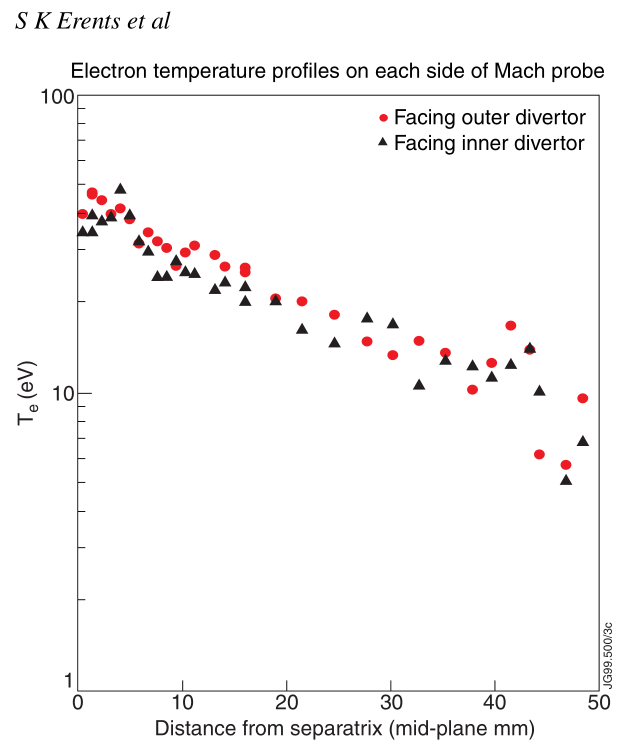
\includegraphics[width=.4\textwidth]{images/jet_sol_parameters.png}
\label{jetsolparams}
\caption{Electron temperatures at JET SOL on each side of a probe. Conditions: $I_p = 2.4$ MA, $B_T = 2.5$ T, $\left< n_e \right> = 2.1 \times 10^{19}$ m$^{-3}$ and $2 MW$ of NBI heating \cite{Erents2002}.}
\end{figure}

During the thesis, we will look for the best methodology to incorporate the relevant parallel kinetic effects in the SOL.

%----------------------------------------------------------------------------------------
%	Objectives
%----------------------------------------------------------------------------------------

\section{Objectives \label{obj}}

The main objective of my thesis is to derive a hybrid kinetic-fluid model applicable in the SOL of magnetic confinement fusion devices.

%----------------------------------------------------------------------------------------
%	Objectives
%----------------------------------------------------------------------------------------

\section{State of the Art \label{firstres}}

Here we shall present a review of hybrid kinetic-fluid models, pointing out which ones are suitable for SOL modeling. Starting from a fluid perspective, the starting model is the drift-reduced Braginskii one (as pointed out above) which states that the heat flux $q_j$ for the particle species $j$ in the collision dominated regime is \cite{Braginskii1965}

\begin{equation}
\vv q_i=-k_\parallel^i \vv b \nabla_\parallel T_i + k_\perp^i \vv b \times \nabla_\perp T_i,
\end{equation}

\begin{equation}
\vv q_e=-0.71 T_e \vv b j_\parallel/e -k_\parallel^e \vv b \nabla_\parallel T_e + k_\perp^e \vv b \times \nabla_\perp T_e,
\end{equation}

\noindent where $k_\parallel^i = 3.9 \frac{n_i T_i \tau_i}{m_i}$, $k_\perp^i=\frac{5 n_i T_i}{2 m_i \omega_{ci}}$, $k_\parallel^e=3.2\frac{n_e T_e \tau_e}{m_e}$ and $k_\perp^e=\frac{5 p_e}{2 m_e \omega_{ce}}$.%----------------------------------------------------------------------------------------
%	Milestones
%----------------------------------------------------------------------------------------

\section{Milestones}

With the objectives defined in section \ref{obj} and considering the time span of 3 years to complete the work, we propose the following road-map 

\begin{itemize}
\item Choose an already used kinetic-fluid model or decide to derive a new one - 6 months
\item Finalize the SOL kinetic-fluid theory - 6 months
\item Incorporate the model in the GBS code - 9 months
\item Run simulations and analyze results - 12 months
\item Write the thesis - 3 months
\end{itemize}

%----------------------------------------------------------------------------------------
%	Miscellaneous
%----------------------------------------------------------------------------------------

\section{Miscellaneous}

\subsection{Conferences}
\begin{itemize}
\item 2015: EFTC (European Fusion Theory Conference)
\item 2016: EPS  (European Physical Society)
\item 2017: EFTC
\item 2018: APS (American Physical Society)
\end{itemize}

\subsection{Courses}

\begin{itemize}
\item Advanced Computation in Physics and Engineering (Fall 2015 - 7.5 ECTS)
\end{itemize}

%----------------------------------------------------------------------------------------
%	References
%----------------------------------------------------------------------------------------

\bibliographystyle{unsrt}
\bibliography{library}

\end{document}